\chapter{ADC Design Using Ideal Circuit Blocks}
After defining all of the architectural features of the design, the next step was to use ideal circuit blocks to simulate the entire ADC design. Designing in this manner gave valuable insights into how different circuit block 
specifications affected overall ADC performance. This chapter begins with an explanation of the ideal circuit blocks that were used in this design. It follows with a discussion of the design and simulated results from a single-ended version of the ADC. This chapter concludes with a discussion of the design of the fully differential ADC and its simulated performance.
\section{Ideal Circuit Blocks}
A set of ideal circuit blocks were provided by Dr. Nan Sun for this design. These circuit blocks include a single-ended OTA, a differential OTA, a comparator, a switch, a clock generator, and a single-ended to differential 
signal converter. This section discusses these blocks in more detail, with input/output details as well as settable parameters.
\subsection{OTA}
The OTA model is used in the design of the first-stage MDAC. The single-ended and differential OTA models are essentially the same, the difference between the two being that the differential model has an additional output pin for the negative output voltage. The pins for the OTA models are given in Table \ref{tab:otapins}.
\begin{table}[htbp]
\begin{center}
\begin{tabular}{|l|l|l|}
\hline
Name & Pin Type & Description \\ \hline
Vdd & Supply & DC power supply \\ \hline
Vin & Input & Positive input voltage \\ \hline
Vinb & Input & Negative input voltage \\ \hline
Vcmo & Output & Common-mode output voltage \\ \hline
Vout & Output & Positive output voltage \\ \hline
Voutb & Output & Positive output voltage, differential model only \\ \hline
\end{tabular}
\end{center}
\caption{OTA Ideal Model Pins}
\label{tab:otapins}
\end{table}
The differential model has an internal common-mode feedback (CMFB) circuit that ensures the common-mode output of the OTA matches the voltage on \emph{Vcmo}. In this design, the power supply is 1.8V. 

In addition to the pins, the OTA models also have a number of parameters that govern its behavior. These parameters are given in Table \ref{tab:otaparams}
\begin{table}[htbp]
\begin{center}
\begin{tabular}{|l|l|}
\hline
Parameter & Description \\ \hline
Gain & OTA DC gain \\ \hline
f\textsubscript{T} & Transistor transit frequency \\ \hline
g\textsubscript{m}/I\textsubscript{d} & Current efficiency \\ \hline
g\textsubscript{m} & Transistor transconductance \\ \hline
noiseconst & Constant controlling total noise power \\ \hline
\end{tabular}
\end{center}
\caption{OTA Ideal Model Parameters}
\label{tab:otaparams}
\end{table}
The device characteristics that are controlled by these parameters are the output voltage, the input capacitance, and the input-referred noise. The \emph{Gain} parameter is the ratio of the output voltage to the input voltage. The input capacitance of the OTA is:
\begin{equation}
C_{in} = \dfrac{g_{m}}{2\pi\cdot f_{T}}
\end{equation}
where $g_{m}$ and $f_{T}$ are OTA parameters. This relationship is based on Equation \ref{eq:transitfrequency}. An internal current source generates current based on the \emph{$g_{m}$/$I_{d}$} and \emph{$g_{m}$} parameters. The input-referred noise of the OTA is:
\begin{equation}
\label{eq:idealotanoise}
\dfrac{\overline{v_{n}^{2}}}{\Delta f} = \dfrac{4\cdot kT\cdot\emph{noiseconst}}{\emph{$g_{m}$}}
\end{equation}
where \emph{noiseconst} and \emph{$g_{m}$} are OTA parameters.
\subsection{Comparator}
The pins for the ideal comparator model are given in Table \ref{tab:comppins}.
\begin{table}[htbp]
\begin{center}
\begin{tabular}{|l|l|l|}
\hline
Name & Pin Type & Description \\ \hline
Vin & Input & Positive input voltage \\ \hline
Vinb & Input & Negative input voltage \\ \hline
CLK & Input & Clock signal \\ \hline
d & Output & Digital decision \\ \hline
db & Output & Logical not of db \\ \hline
\end{tabular}
\end{center}
\caption{Comparator Ideal Model Pins}
\label{tab:comppins}
\end{table}
When \emph{CLK} = 0V, the comparator operates in a tracking mode. In this mode, the input voltages are sampled onto capacitors inside the model. When \emph{CLK} = 1.8V, the comparator goes into its decision phase. In the decision phase, the output \emph{d} is given by:
\begin{equation}
\emph{d} = \begin{cases}
				1 & \mbox{if } V_{in} > V_{inb} \\
				0 & \mbox{if } V_{in} < V_{inb}
			\end{cases}
\end{equation}
\subsection{Clock Generator}
The clock generator is used to generate the non-overlapping clocks for the design. The pins for this block are given in Table \ref{tab:clkgenpins}.
\begin{table}[htbp]
\begin{center}
\begin{tabular}{|l|l|l|}
\hline
Name & Pin Type & Description \\ \hline
f1 & Output & $\phi_{1}$ clock signal \\ \hline
f1e & Output & $\phi_{1}$ clock signal with early falling edge \\ \hline
f2 & Output & $\phi_{2}$ clock signal \\ \hline
f2e & Output & $\phi_{2}$ clock signal with early falling edge \\ \hline
f1b & Output & Complementary $\phi_{1}$ clock signal \\ \hline
f1eb & Output & Complementary $\phi_{1}$ clock signal with early falling edge \\ \hline
f2b & Output & Complementary $\phi_{2}$ clock signal \\ \hline
f2eb & Output & Complementary $\phi_{2}$ clock signal with early falling edge \\ \hline
\end{tabular}
\end{center}
\caption{Ideal Clock Generator Pins}
\label{tab:clkgenpins}
\end{table}
The parameters that control the behavior of these outputs are given in Table \ref{tab:clkgenparams}.
\begin{table}[htbp]
\begin{center}
\begin{tabular}{|l|l|}
\hline
Parameter & Description \\ \hline
period & Clock period \\ \hline
t\_early & Time difference between the falling edge of f1 and f1e \\ \hline
t\_edge & The rise and fall times \\ \hline
t\_nonoverlap & The non-overlapping time between f1 and f2 \\ \hline
\end{tabular}
\end{center}
\caption{Ideal Clock Generator Parameters}
\label{tab:clkgenparams}
\end{table}
\subsection{Switch}
The switch model has three pins, given in Table \ref{tab:switchpins}
\begin{table}[htbp]
\begin{center}
\begin{tabular}{|l|l|l|}
\hline
Name & Pin Type & Description \\ \hline
A & Input/Output & One side of switch \\ \hline
B & Input/Output & One side of switch \\ \hline
ctrl & Input & Control input \\ \hline
\end{tabular}
\end{center}
\caption{Ideal Switch Pins}
\label{tab:switchpins}
\end{table}
The switch is open when the voltage on the \emph{ctrl} pin is less than 0.9V. When the voltage on \emph{ctrl} is greater than 0.9V, the switch is closed and \emph{A} is connected to \emph{B}. The switch has only one parameter, given in Table \ref{tab:switchparams}.
\begin{table}[htbp]
\begin{center}
\begin{tabular}{|l|l|}
\hline
Parameter & Description \\ \hline
ron & Closed switch resistance \\ \hline
\end{tabular}
\end{center}
\caption{Ideal Switch Parameters}
\label{tab:switchparams}
\end{table}
\subsection{Single-to-Differential Converter}
This block takes in a single-ended signal along with a common-mode voltage and outputs a differential voltage. The pins for the single-to-differential converter are given in Table \ref{tab:s2dpins}
\begin{table}[htbp]
\begin{center}
\begin{tabular}{|l|l|l|}
\hline
Name & Pin Type & Description \\ \hline
Vin & Input & Single-ended input voltage \\ \hline
Vcmi & Input & Common-mode input voltage \\ \hline
Vout & Output & Positive output voltage \\ \hline
Voutb & Output & Negative output voltage \\ \hline
\end{tabular}
\end{center}
\caption{Ideal Single-Ended-to-Differential Converter Pins}
\label{tab:s2dpins}
\end{table}
The relationship between the output voltages and the input voltage is:
\begin{align}
\label{eq:s2d}
V_{out} = V_{cmi} + \dfrac{V_{in}}{2} \\[0.5em]
\nonumber V_{outb} = V_{cmi} - \dfrac{V_{in}}{2}
\end{align}
\section{Calculation of Design Parameters}
\label{sec:designparameters}
Before any schematic entry or simulation could be performed, the required design parameters needed to be calculated. These correspond to the parameters of the ideal circuit blocks, as well as the size of the capacitors for both pipeline stages. A Matlab script was used to perform all of the calculations outlined in this section.
\subsection{Calculation of Capacitor Size}
The main factor determining the required capacitor size is thermal noise. As mentioned in Section \ref{sec:saraccuracy} most designs try to obtain thermal noise that is on the order of quantization noise. In order to achieve this, the noise power has to be partitioned between all of the noise sources. In the case of this design, the noise sources are the first and second stage capacitive arrays and the OTA. The partitioning chosen for this design was 45\% of total noise power allotted to the first stage capacitor array, 45\% for the OTA, and 10\% for the second stage capacitive array. The reasoning behind allotting such a small percentage to the second stage capacitive array is that the output noise of the second stage will be divided by the closed loop gain of the MDAC, 16, when calculating input-referred noise. Having such a large closed loop gain should mean that the effect of the second stage thermal noise on overall quantization noise should be very small. For a 12 bit ADC with a full-scale voltage of 2V, the quantization noise power is \SI{141}{\micro\volt_{rms}}. Using this value, the maximum noise calculations in Table \ref{tab:maxinputnoise} can be obtained.
\begin{table}[htbp]
\centering
\begin{tabularx}{\linewidth}{|X|l|X|}
\hline
Noise Source & Noise Power (\si{\square\nano\volt}) & RMS Noise Voltage (\si{\micro\volt_{rms}}) \\ \hline
12 bit ADC Quantization Noise & 19.9 & 141 \\ \hline
Stage 1 Capacitors & 8.94 & 94.6 \\ \hline
OTA & 8.94 & 94.6 \\ \hline
Stage 2 Capacitors & 1.99 & 4.46 \\ \hline
\end{tabularx}
\caption{Maximum Input Referred Noise}
\label{tab:maxinputnoise}
\end{table}
While input-referred noise is the metric used for calculating SNDR, most measurements obtain the output-referred noise. For this reason, it is also useful to look at the maximum output-referred noise for each of these noise generators. In an effort to balance the total noise contribution with the required power consumption, the maximum output-referred noise for the second stage was scaled by a factor of $A_{cl}$ instead of the typical $A_{cl}^{2}$~\cite{315breader}. The output-referred noise calculations are summarized in Table \ref{tab:maxoutputnoise}. 
\begin{table}[htbp]
\begin{center}
\begin{tabularx}{\linewidth}{|X|l|X|}
\hline
Noise Source & Noise Power (\si{\square\micro\volt}) & RMS Noise (\si{\milli\volt_{rms}}) \\ \hline
Stage 1 Capacitors & 2.29 & 1.5 \\ \hline
OTA & 2.29 & 1.5 \\ \hline
Stage 2 Capacitors & 0.318 & 0.1783 \\ \hline
\end{tabularx}
\caption{Maximum Output Referred Noise}
\label{tab:maxoutputnoise}
\end{center}
\end{table}

With the maximum noise power for the capacitive arrays defined, the sizes of the capacitors could be calculated. Figure \ref{fig:generalmdac} is a simplified model of the MDAC used in this design.
\begin{figure}[htb]
\centering
\newcommand{\xswitchright}{2}
\newcommand{\csoneright}{\xswitchright+1}
\newcommand{\xmdacin}{\csoneright+1}
\newcommand{\xmdacout}{\xmdacin+4}
\newcommand{\rowone}{0}
\newcommand{\rowtwo}{\rowone-1.5}
\newcommand{\rowthree}{\rowtwo-1.25}
\newcommand{\rowfour}{\rowthree-1}
\begin{circuitikz} 
\draw
	(0,0) node[anchor=east]{$V_{in}$}
	%sample switch 1
		to [cspst, l=$S$] (\xswitchright,0)
		to [short, -*] (\xswitchright, 0)
	%cs1
		to [C, l=$C_{s1}$] (\csoneright, 0)
		to [cspst, -*, l=$\phi_{2}$] (\xmdacin, 0)
		to [short, -*] (\xmdacin, 0)
		node[anchor=south west] {X}
		to [short, -*] (\xmdacin, 1)
	%cf
		to [C, l=$C_f$] (\xmdacout, 1) to [short, -*] ++(0, 0)
	%feedback switch
		(\xmdacin, 1) -- (\xmdacin, 2.2) to [cspst, l=$\phi_{1}$] (\xmdacout, 2.2) -- (\xmdacout, 1)
	%ota
		(\xmdacin+1, \rowone) node[op amp, anchor=-] (ota) {}
		(ota.+) -| ++(-0.25, -.25) node[ground] {}
		(\xmdacin, \rowone) -- (ota.-)
		(ota.center) ++(-0.1,0) node[anchor=center] {OTA}
	%Vdac switch
	(0, \rowtwo) node[anchor=east] {$V_{DAC}$}
		to [cspst, l=$\phi_{2}$] (\xswitchright,\rowtwo)
		(\xswitchright, \rowtwo) -- (\xswitchright, \rowone)
	%phi1e switch
		(\xmdacin, \rowone) -- (\xmdacin, \rowtwo) to [cspst, l=$S_{e}$] (\xmdacin, \rowthree)
		(\xmdacin, \rowthree) node[ground] {}
		(ota.out) -| (\xmdacout, 1) 
		(ota.out) ++(0.62,0) to [short, *-] ++(0,0) to [cspst, l=$\overline{\phi_{2}}$] ++(0,-1)
		node[ground] {}
		(ota.out) --  ++(2, 0) node[above] {$V_{res,o}$}
	%cl
		to [C, l=$C_{s2}$] ++(0, -1)
		node[ground] {}
;
\end{circuitikz}
\caption{Simplified Schematic of MDAC}
\label{fig:generalmdac}
\end{figure}
In this figure, the capacitive arrays for both stages are lumped into single capacitors, $C_{s1}$ and $C_{s2}$. An additional feedback capacitor, $C_{f}$, sets the closed loop gain of the MDAC. The expression for the closed loop gain is:
\begin{align}
\label{eq:mdacacl}
A_{cl} &= -\dfrac{C_{s1}}{C_{f}} \\
\nonumber &= 16
\end{align}
In addition, the SAR control logic, switches, and comparator are abstracted away as a final output voltage, $V_{DAC}$, that is applied to $C_{s1}$ during $\phi_{2}$. Also, the sampling switches are labeled with $S$ instead of $\phi_{1}$ to signify that $\phi_{1}$ is now split into a sampling and conversion phase. During the sampling phase, the OTA is no longer connected to the input capacitance, and thus has no effect on the output noise. An equivalent schematic for the MDAC in the sampling phase is given in Figure \ref{fig:mdacsampling}.
\begin{figure}[htb]
\centering
\newcommand{\nextcol}{1.3}
\newcommand{\nextrow}{1.3}
\newcommand{\halfrow}{\nextrow/2}
\newcommand{\halfcol}{\nextcol/2}
\begin{circuitikz}
\draw
	(0, 0) node[anchor=east] {$V_{in}$} -- ++(\halfcol, 0)
%input switch
	to [R] ++(\nextcol, 0)
	to [C, l=$C_{s1}$] ++(\nextcol, 0) to [short, *-] ++(0, 0) -- ++(0, -\halfrow)
	node[anchor=south west] {X}
	to [R] ++(0, -\nextrow)
	node[ground] {}
	(2*\nextcol+\halfcol, 0) -- ++(0,\nextrow)
	to [C, l=$C_{f}$] ++(\nextcol, 0)
	to [R] ++(\nextcol, 0) -- ++(\halfcol, 0)
	node[ground] {}
;\end{circuitikz}
\caption{Equivalent MDAC Schematic in the Sampling Phase}
\label{fig:mdacsampling}
\end{figure}
In this configuration, the output-referred noise is~\cite{315breader}:
\begin{align}
\label{eq:samplingoutputnoise}
\overline{v_{o}^{2}} &= \dfrac{\overline{q}_{x}^{2}}{C_{f}^{2}} \\[0.5em]
\nonumber	&= \dfrac{kT(C_{s1}+C_{f})}{C_{f}^2} \\[0.5em]
\nonumber	&= \dfrac{kT}{C_{f}}\left(1+\dfrac{C_{s1}}{C_{f}}\right) \\[0.5em]
\nonumber	&= \dfrac{16kT}{C_{s1}}\cdot(17) \\[0.5em]
\nonumber	&= (0.5)\cdot(\SI{2.29}{\square\micro\volt})
\end{align}
where the relationship from Equation \ref{eq:mdacacl} was used to put the equation in terms of $C_{s1}$. Since this calculation only accounts for the single-ended noise contribution from $C_{s1}$, the maximum output noise power was multiplied by a factor of $\nicefrac{1}{2}$. Solving Equation \ref{eq:samplingoutputnoise} for $C_{s1}$ yields:
\begin{align}
\label{eq:cs1size}
C_{s1} &= \dfrac{16kT\cdot 17}{(0.5)\cdot(\SI{2.29}{\square\micro\volt})} \\[0.5em]
\nonumber	&= \SI{976.3}{\femto\farad}
\end{align}
Using Equation \ref{eq:ctot}, the stage 1 unit capacitance is:
\begin{align}
\label{eq:cu1size}
C_{u1} &= \dfrac{C_{s1}}{2^{(6-1)}}\\
\nonu	&= \SI{30.51}{\femto\farad}
\end{align}
Using the value of $C_{s1}$ in Equation \ref{eq:mdacacl}, the feedback capacitance is:
\begin{align}
C_{f} &= \dfrac{\SI{976.3}{\femto\farad}}{16} \\[0.5em]
\nonu &= \SI{61.02}{\femto\farad}
\end{align}
The only contribution from the second stage capacitance to the total output-referred noise is kT/C noise. The expression for $C_{s2}$ in terms of maximum output noise power is:
\begin{align}
\label{eq:cs2sizetemp}
C_{s2} &= \dfrac{kT}{\overline{v}_{on,max}^2} \\
\nonu &= \SI{129.3}{\femto\farad}
\end{align}
From Equation \ref{eq:ctot}, $C_{u2}$ is calculated to be \SI{2.02}{\femto\farad}. This value, unfortunately, is well under the minimum MIMcap capacitor size allowed by the \SI{180}{\nano\meter} technology, which is \SI{20.28}{\femto\farad}. Using the minimum unit capacitance, the value of $C_{s2}$ is:
\begin{align}
\label{eq:cu2size}
C_{s2} &= 2^{7-1}\cdot(\SI{20.28}{\femto\farad}) \\
\nonu	&= \SI{1.30}{\pico\farad}
\end{align}
The values for $C_{s1}$, $C_{s2}$, and $C_{f}$ fully specify the capacitances of this design.

With unit capacitance values for both stages calculated, the statistical mismatch could be calculated to ensure that it was within reasonable bounds. Table \ref{tab:capmismatch} summarizes the statistical effect of mismatch on the DNL and INL of each stage. The mismatch standard deviation, $\sigma_{u}$ was calculated from foundry data.
\begin{table}[htbp]
\centering
\begin{tabular}{|r|r|r|r|r|}
\hline
Stage & Resolution (bits) & $\sigma_{u}$ & $\sigma_{DNL}$ (LSB) & $\sigma_{INL}$ (LSB) \\ \hline
1 & 6 & 0.0036 & 0.0144 & 0.0286 \\ \hline
2 & 7 & 0.00028 & 0.0016 & 0.0032 \\ \hline
\end{tabular}
\caption{Capacitor Mismatch Effect on ADC INL and DNL}
\label{tab:capmismatch}
\end{table}
From these calculations, it can be seen that the capacitor mismatch has a minimal effect on INL and DNL.
\subsection{Calculation of OTA Model Parameters}
\label{sec:idealotaparams}
Once noise partitioning and the calculation of the capacitor sizes was performed, all of the OTA model parameters could be calculated. First, the required OTA gain was calculated, followed by the \gmid\spc and the transit 
frequency. Finally, a calculation of the required OTA bandwidth was performed, which was used to calculate the required OTA transconductance. 

The required OTA loop gain is determined by the specified static gain error that is presented to the ADC. The static gain percentage, \es, in terms of OTA loop gain is~\cite{315areader}:
\begin{equation}
\label{eq:es}
\epsilon_{s} = \dfrac{1}{T_{0}}
\end{equation} 
where \tnot\spc is the OTA loop gain. For a single-stage OTA, the relationship between \tnot\spc and the OTA open-loop gain is:
\begin{align}
\label{eq:loopgain}
T_{0} &= \beta G_{m} R_{o} \\
\nonu &= \beta A_{OLDC}
\end{align}
where \Gm\spc is the transconductance of the OTA, \Ro\spc is the OTA output resistance, and $A_{OLDC}$ the OTA open loop gain. The \Gain\spc OTA parameter is equivalent to $A_{OLDC}$. 
For the static error to not have a significant effect on the accuracy of the downstream ADC, the static error was decided to be $\nicefrac{1}{2}$ LSB. To obtain this, the expression for \es\spc is:
\begin{align}
\label{eq:eshalflsb}
\epsilon_{s} &= \dfrac{\Delta_{2}}{2\cdot V_{FS,2}} \\
\nonu &= 0.0039
\end{align}
where $\Delta_{2}$ is the LSB size of the second stage ADC, and $V_{FS,2}$ is the full-scale voltage of the second stage. The full-scale voltage of the second stage is reduced to 1V by the usage of the half-gain MDAC. Using Equations \ref{eq:eshalflsb} and \ref{eq:es}, the required loop gain is: 
\begin{align}
\label{eq:loopgaincalc}
T_{0} &= \dfrac{1}{\epsilon_{s}} \\[0.5em]
\nonu &\approx 256 \\
\nonu &\approx \SI{48}{\decibel}
\end{align}
Using Equations \ref{eq:loopgain} and \ref{eq:loopgaincalc}, the required open-loop gain is:
\begin{align}
\label{eq:otagain}
A_{OLDC} &= \dfrac{1}{\epsilon_{s}\cdot\beta} \\
\nonu &\approx 4352 \\
\nonu &\approx \SI{73}{\decibel}
\end{align}
Interestingly, this value holds for any 12 bit pipelined ADC regardless of its stage resolutions. For each additional bit resolved in the second stage, the feedback factor and the LSB size increases by a factor of approximately two, so the overall open-loop gain requirement remains unchanged. Once the required open-loop gain has been determined, some assumptions had to be made about the implementation of the OTA in order to calculate \gmgds, \gmid, and \transit. The assumption made for this design was that a triple-cascoded amplifier would be used. Cascode topologies are very power efficient due to their load compensation~\cite{5595209}. The load compensation also makes designing a stable amplifier a less challenging task. Finally, for the same \gmgds, a cascode provides more gain than a two-stage amplifier. The main limitation of cascode devices is their lower output swing. This design mitigates this issue through the use of the half-gain MDAC. The gain of a triple-cascode is approximately:
\begin{equation}
\label{eq:triplecascodegain}
A_{OLDC} = \dfrac{1}{2}\left(\dfrac{g_{m}}{g_{ds}}\right)^{3}
\end{equation}
From Equation \ref{eq:triplecascodegain}, the required \gmgds\spc is calculated to be 20.57. From the \gmid\spc lookup functions mentioned in Section \ref{sec:gmid}, the \gmid\spc OTA parameters is 4.0325 and the \transit\spc OTA parameter is \SI{45.5}{\giga\hertz}. The \gmid\spc specified for this design was probably too low for a practical design, since \gmid\spc is inversely proportional to the transistor overdrive voltage. Increasing \gmid\spc in the actual implementation would decrease the static error, so the this issue would not constrain the static error. Increasing \gmid\spc does decrease the transit frequency, which means larger parasitic capacitances. Once $g_{m}$ was calculated, the effect of raising \gmid\spc on parasitic capacitance could be more fully explored.

In order to calculate the required OTA transconductance, the allowable dynamic error must be specified. The dynamic output error is directly tied to the bandwidth of the OTA. For this design, it was desired to settle to within \nicefrac{1}{8} LSB of the second stage in a half clock cycle. The OTA loop crossover frequency in terms of dynamic error is~\cite{315areader}:
\begin{align}
\label{eq:fcdynamicerror}
f_{c} &= \left(\dfrac{-f_{s}}{\pi}\right)\ln\left(\epsilon_{d}\left[1-\beta\dfrac{C_{f}}{C_{f}+C_{s2}}\right]\right) \\[0.5em]
\nonu &= \left(\dfrac{-\SI{10}{\mega\hertz}}{\pi}\right)\ln\left(\dfrac{1}{8\cdot2^{7}}\left[1-\dfrac{1}{17}\cdot\dfrac{\SI{61}{\femto\farad}}{\SI{61}{\femto\farad}+\SI{1.3}{\femto\farad}}\right]\right) \\[0.5em]
\nonu &= \SI{22.1}{\mega\hertz}
\end{align}
where $f_{s}$ is the sampling frequency and \ed\spc is the tolerable dynamic error. The loop-crossover frequency is equivalent to the \SI{-3}{\decibel} bandwidth of the closed loop MDAC. The expression in Equation \ref{eq:fcdynamicerror} purposefully ignores the effects of slewing on settling time. Slewing occurs when the differential output current saturates to to large differential input voltage steps. During slew time, the amplifier output is driven with an approximately constant current bias that is equal to the tail bias. For the amplifier to operate in this condition, the input differential voltage, $V_{id}$ must be:
\begin{equation}
\label{eq:slewinputdiff}
|V_{id}| > \sqrt{2}\cdot V_{ov}
\end{equation}
where $V_{ov}$ is the overdrive voltage of the input transistor. From long-channel equations, $V_{ov}$ is approximately:
\begin{equation}
\label{eq:vov}
V_{ov} \approx \dfrac{2}{g_{m}/I_{d}}
\end{equation}
The maximum differential input voltage step for a design is limited by its closed-loop gain and the absolute value of its maximum differential output voltage. An expression for the maximum $V_{id}$ in terms of these values is:
\begin{equation}
\label{eq:vidmax}
|V_{id,max}| = \dfrac{|V_{od,max}|}{A_{cl}} 
\end{equation}
where $V_{od,max}$ is the maximum differential output voltage and $A_{cl}$ is the closed-loop gain. Combining Equations \ref{eq:slewinputdiff}, \ref{eq:vov}, and \ref{eq:vidmax}, solving for \gmid, and plugging in values for this design, the maximum \gmid\spc that can be used without slewing is:
\begin{align}
\label{eq:maxgmid}
(g_{m}/I_{d})_{max} &= \dfrac{2.8\cdot A_{cl}}{|V_{od,max}|} \\[0.5em]
\nonu				&= \dfrac{2.8\cdot16}{1} \\[0.5em]
\nonu				&= \SI{44.8}{\per\volt}
\end{align}
In the weak inversion region, MOSFET operation is very similar to bipolar junction transistor (BJT) operation. The \gmid\spc in weak inversion approximates the \gmid\spc of a BJT with a reduction factor caused by capacitive division on the base potential of the MOSFET. The expression for \gmid\spc of a BJT is: 
\begin{equation}
(g_{m}/I_{d})_{BJT} = \dfrac{1}{V_{T}}
\end{equation}
where $V_{T}$ is the thermal voltage. This corresponds to a \gmid\spc value of approximately \SI{38}{\per\volt} at room temperature. Since \gmid\spc of a MOSFET is always below the \gmid\spc of a BJT, the \gmid\spc value calculated in Equation \ref{eq:maxgmid} is not achievable. For this reason, slewing was ignored in the derivation of the settling time equation. An alternative expression for the closed loop bandwidth in terms of the OTA transconductance is:
\begin{equation}
\label{eq:fc}
f_{c} = \dfrac{\beta G_{m}}{2\pi C_{L,tot}}
\end{equation}
where $C_{L,tot}$ is the total load capacitance of the OTA. In order to calculate \Gm\spc from Equation \ref{eq:fc}, the total load capacitance must be known. An approximate expression for the total load capacitance that neglects OTA parasitics is:
\begin{align}
\label{eq:cltotapprox}
C_{L,tot} &= C_{s2} + (1-\beta)\cdot C_{f} \\
\nonu &= \SI{1.36}{\pico\farad}
\end{align}
Using the calculated load capacitance in Equation \ref{eq:fc} and solving for the OTA transconductance yields:
\begin{align}
\label{eq:idealgm}
G_{m} &= \dfrac{(2\pi f_{c})(C_{L,tot})}{\beta} \\[0.5em]
\nonu &= \SI{3.2}{\milli\siemens}
\end{align}
With \Gm\spc now calculated, the potential effect of raising \gmid\spc on parasitic capacitance could be examined. Table \ref{tab:parcapotagmid} shows the simulated total gate capacitance for a number of \gmid\spc values.
\begin{table}[htbp]
\centering
\begin{tabular}{|r|r|}
\hline
\multicolumn{1}{|l|}{$g_{m}/I_{d}$} & \multicolumn{1}{l|}{$C_{gg}$ (\ff)} \\ \hline
10 & 19 \\ \hline
15 & 32.7 \\ \hline
20 & 75 \\ \hline
22 & 133 \\ \hline
\end{tabular}
\caption{Total Gate Capacitance for Given $g_{m}$/$I_{d}$}
\label{tab:parcapotagmid}
\end{table}
For the total gate capacitance to be 10\% of the load capacitance, \gmid\spc has to be set to larger than 22. This gives adequate design headroom so that the unrealistic \gmid\spc used for the ideal design was not given further consideration.

The final OTA parameter that needed to be calculated was the \emph{noiseconst}. The expression for the noise of a basic cascode stage is~\cite{315areader}:
\begin{equation}
\label{eq:cascoutputnoise}
\overline{v_{o}^{2}} = \dfrac{1}{\beta}\gamma\left(1+\dfrac{g_{m2}}{g_{m1}}\cdot\dfrac{\omega_{c}}{\omega_{p2}}\right)
\end{equation}
where $g_{m2}$ is the transconductance of the common-gate transistor, $g_{m1}$ is the transconductance of the common-source transistor, $\gamma$ is a parameter that is a function of transistor parameters and bias conditions, and $\omega_{p2}$ is the non-dominant pole frequency. In order to simplify this expression to a constant, some approximations need to be made. First, the parameter $\gamma$ is assumed to be 1, which is a reasonable approximation for short channel devices~\cite{1202575}. Next, for optimal settling performance, a phase margin of 75$\deg$ is assumed. This constraint means that the ratio of $\omega_{p2}$ to $\omega_{c}$ is 3:1. Finally $g_{m1}$ and $g_{m2}$ are assumed to be approximately equal. Using these approximations, dividing both sides of the expressions by the equivalent noise bandwidth, and referring the noise to the input gives the expression:
\begin{align}
\label{eq:noiseconstexpression}
\dfrac{\overline{v_{i}^{2}}}{\Delta f} &= kT\dfrac{\left(\dfrac{1}{1.57\beta^{2}}+\dfrac{1}{4.71\beta^{2}}\right)\cdot 2\pi}{A_{cl}^{2}\cdot g_{m}} \\[0.5em]
\nonu &= \dfrac{6.02kT}{g_{m}}
\end{align}
Another abstraction used in this simplification is that this only includes noise sources from a basic cascode stage, not from a triple-cascode. To allow for some headroom from the additional noise of the additional common-gate transistor, a factor of 1.5 was applied to the input-referred noise. Applying this factor, setting Equations \ref{eq:noiseconstexpression} and \ref{eq:idealotanoise} equal to each other, and solving for \emph{noiseconst} yields a \emph{noiseconst} value of 2.36. Using the calculated $g_{m}$, the total input-referred OTA noise is \SI{20.5}{\micro\volt_{rms}}. Comparing this value to that from Table \ref{tab:maxinputnoise}, the calculated value is well below the maximum input-referred noise, so even if these approximations yielded an optimistic approximation, there was plenty of additional noise headroom to compensate.

Table \ref{tab:otasetparams} summarizes the OTA parameters that were used for the ideal design.
\begin{table}[htbp]
\renewcommand*\arraystretch{1.3}
\centering
\begin{tabular}{|l|r|}
\hline
Parameter & \multicolumn{1}{l|}{Value} \\ \hline
Gain & 4352 \\ \hline
$f_{T}$ & \num{4.55e10} \\ \hline
$g_{m}$/$I_{d}$ & 4.0325 \\ \hline
$g_{m}$ & 0.0033 \\ \hline
noiseconst & 2.36 \\ \hline
\end{tabular}
\caption{Parameter Settings for Ideal OTA Model}
\label{tab:otasetparams}
\end{table}
\subsection{Switch Parameters}
The only parameter that needed to be set for the ideal switch was its closed resistance. Generally one should strive for a switch RC that is 10 times or greater than the bandwidth of the OTA. The distributed nature of the switches and capacitors made obtaining a numerical expression for the ideal switch resistance difficult. It was decided to start at a low resistance of \SI{100}{\ohm} and increase the resistances until it began affecting system performance.
\subsection{Clock Generators}
A number of clock domains were needed for this design. Many of these clocks also had to be gated so that they only operated in one phase of the main clock. The main clock generator was used to generate the $\phi_{1}$ and $\phi_{2}$ signals. Another clock generator was used to generate the sampling clocks. Two additional clock generators were needed to control the SAR clocks. The required period for the SAR clocks was calculated using Equation \ref{eq:compdecisiontimegiventsamp}. Table \ref{tab:clockingscheme} summarizes all of the clock signals in the design, their frequencies, and the signals that were used to gate the clocks.
\begin{table}[htbp]
\begin{center}
\renewcommand*\arraystretch{1.3}
\begin{tabularx}{\linewidth}{|l|l|X|l|}
\hline
Clock Signal & Clock Frequency & Description & Gating Signals \\ \hline
$\phi_{1}$ & \SI{10}{\mega\hertz} & Phase 1 of \SI{10}{\mega\hertz} clock & N/A \\ \hline
$\phi_{2}$ & \SI{10}{\mega\hertz} & Phase 2 of \SI{10}{\mega\hertz} clock & N/A \\ \hline
S & \SI{20}{\mega\hertz} & Sampling clock, used to control sampling switches & $\phi_{1}$ \\ \hline
comp1clk & \SI{240}{\mega\hertz} & Stage 1 SAR Clock & $\overline{S}, \phi_{1}$ \\ \hline
comp2clk & \SI{140}{\mega\hertz} & Stage 2 SAR Clock & $\phi_{2}$ \\ \hline
\end{tabularx}
\end{center}
\caption{Design Clocks}
\label{tab:clockingscheme}
\end{table}
Figure \ref{fig:basicclocks} shows a general waveform of  a single cycle of the design clocks and how the signals relate to each other.
\begin{figure}[htbp]
\centering
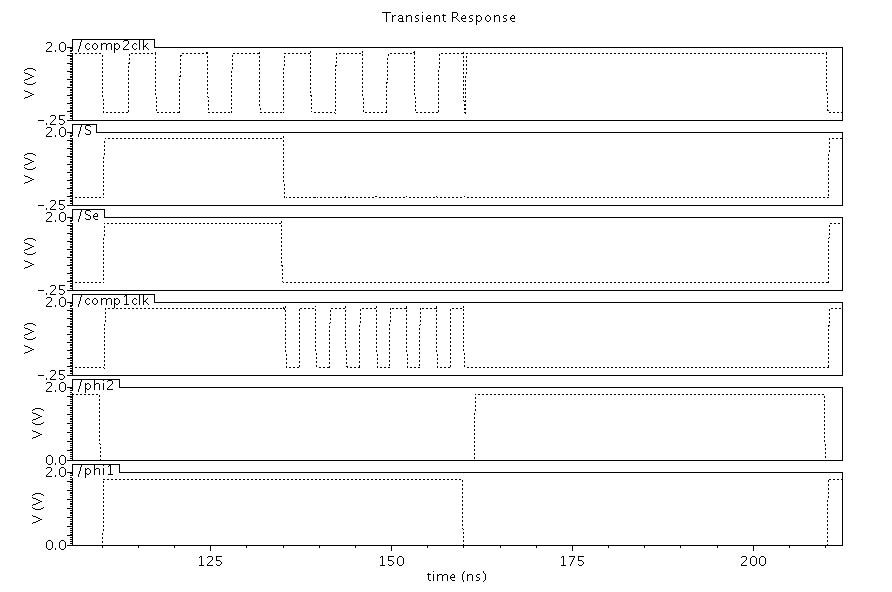
\includegraphics[width=\textwidth]{basicclocks}
\caption{Waveform of a Single Cycle of Design Clocks}
\label{fig:basicclocks}
\end{figure}
\section{Design of Single-Ended ADC}
With the calculation of all the general design parameters complete, the design could move into the circuit design and simulation phase. The first design was a single-ended one, as this design was easier to debug. Although all of the previous chapter's calculations assumed a differential design, only a few changes needed to be made to accommodate the single-ended design. First, the full-scale voltage would only be \SI{1}{\volt} for the single-ended design. Second, all noise calculations were done assuming differential capacitor arrays, so expected noise contributions had to be halved for the single-ended design. The operation of the first and second stage SAR ADCs follows the explanation in Section \ref{sec:saroperation}, with the operation expanded to six and seven bits, respectively. The first task in the single-ended design was to design the digital SAR control logic. Next, the clocking scheme, capacitor sizes, and digital logic were verified by using ideal component parameters. Once all of the surrounding logic had been verified, the calculated parameters from Section \ref{sec:designparameters} were put into the ideal models. With the calculated parameters, transient simulations were run to verify that the MDAC settling met the specifications from Section \ref{sec:idealotaparams}. Once adherence to the settling specification was verified, a longer simulation was run to obtain device SQDR. Once the 74 dB SQDR was achieved, noise simulations were run to ensure that the total input-referred noise met the design specifications. Once all this was complete, work moved on to the differential design.
\subsection{Single-Ended SAR Control Logic}
The SAR control logic determines the operation of all of the conversion switches in the design. In addition, it uses the comparator output to construct the digital output code of the ADC. All of the digital logic described in this section was designed at the gate level using standard cells. Due to the low speed, in digital terms, of the clocks in this design and the low complexity of the digital logic, minimum sized gates were used throughout the design. Using minimum sized gates decreases the dynamic power consumption of the digital blocks in the design.

The first-stage SAR logic was designed first with the intention of expanding the logic to the second stage. The SAR control logic governs the behavior of the $d_i$ switches in Figure \ref{fig:saradcex}. The first-stage control logic was implemented as a state machine with the negative edge of the SAR clock controlling state transitions. Table \ref{tab:stageonestatemachine} summarizes the operation of the SAR state machine. In this table, $C$ corresponds to the comparator output at the end of the previous state, and $d_ip$ corresponds to the $d_i$ signal maintaining its previous state. 
\begin{table}[htbp]
\renewcommand*\arraystretch{1.3}
\begin{center}
\begin{tabular}{|r|r|r|r|l|r|r|r|}
\hline
\multicolumn{ 2}{|c|}{State Outputs} & \multicolumn{ 6}{c|}{Switch Outputs} \\ \hline
\multicolumn{1}{|l|}{Current State} & \multicolumn{1}{l|}{Next State} & \multicolumn{1}{l|}{$d_{5}$} & \multicolumn{1}{l|}{$d_{4}$} & $d_{3}$ & \multicolumn{1}{l|}{$d_{2}$} & \multicolumn{1}{l|}{$d_{1}$} & \multicolumn{1}{l|}{$d_{0}$} \\ \hline
0 & 1 & 0 & 0 & \multicolumn{1}{r|}{0} & 0 & 0 & 0 \\ \hline
1 & 2 & 1 & 0 & \multicolumn{1}{r|}{0} & 0 & 0 & 0 \\ \hline
2 & 3 & $\overline{C}$ & 1 & \multicolumn{1}{r|}{0} & 0 & 0 & 0 \\ \hline
3 & 4 & $d_{5p}$ & $\overline{C}$ & \multicolumn{1}{r|}{0} & 0 & 0 & 0 \\ \hline
4 & 5 & $d_{5p}$ & $d_{4p}$ & \multicolumn{1}{r|}{$\overline{C}$} & 1 & 0 & 0 \\ \hline
5 & 6 & $d_{5p}$ & $d_{4p}$ & $d_{3p}$ & $\overline{C}$ & 1 & 0 \\ \hline
6 & 7 & $d_{5p}$ & $d_{4p}$ & $d_{3p}$ & \multicolumn{1}{l|}{$d_{2p}$} & $\overline{C}$ & 1 \\ \hline
7 & 0 & $d_{5p}$ & $d_{4p}$ & $d_{3p}$ & \multicolumn{1}{l|}{$d_{2p}$} & \multicolumn{1}{l|}{$d_{1p}$} & $\overline{C}$ \\ \hline
\end{tabular}
\end{center}
\caption{Stage One SAR Control Logic State Machine}
\label{tab:stageonestatemachine}
\end{table}
When the ADC is in the sampling phase, clock signal $S$ is active and all other switches are open. This is accomplished by gating all the $d_{i}$ and $\overline{d_{i}}$ switch control inputs with $\overline{S}$. During this phase, the SAR state machine is reset to its initial state.  Once the sampling phase ends, the first stage SAR clock, \emph{comp1clk}, falls, the state machine moves into State 1, and the SAR begins its conversion operation. For the state machine to complete all of its operations, seven \emph{comp1clk} falling edges are required. Once the state machine reaches State 7, it maintains its state until the next sampling clock rising edge. This state machine must hold its state throughout $\phi_{2}$ so that the residue voltage is properly amplified by the MDAC. Once the sampling clock rising edge occurs, the state machine is reset to State 0, and all of the SAR switches open. 

The SAR control logic for the second stage ADC is almost identical to the first stage. An additional state and digital output were added to accommodate the seven bit ADC. In this case, eight falling \emph{comp2clk} edges are required. Also, the second stage state machine is reset by the negative edge of $\phi_{2}$, which corresponds to the sampling phase of the second stage ADC. Other than these differences, the operation of the second stage SAR is identical to that of the first stage.
\subsection{Test Setups}
\label{sec:adcsimulations}
Before continuing with the discussion on simulating the ADC using ideal component parameters, it is worthwhile to discuss the simulation tests that were used throughout the design of this ADC. When evaluating the performance of the entire pipelined system, four main tests were used for all design iterations. The first was a short transient simulation to ensure that the MDAC output was settling properly and the digital outputs were being set properly. The next test was a longer transient simulation that was used to perform a DFT on the digital output. Once performance in these two simulations met specifications, two different types of noise simulations were run, in order to provide a means of verifying that the noise results were accurate. First, AC noise simulations were run on the ADC in both its sampling and amplification phases. Next, a transient periodic noise simulation was run on the ADC. Once transistor level models for the OTA had been integrated into the full ADC, power consumption simulations were also performed on the design. This section describes in more detail each of these simulations.
\subsubsection{Transient Settling Test}
\label{sec:transettling}
In this test, a full-scale voltage step was applied to the input of the ADC. The digital output was checked to ensure that the output was the maximum digital code from the ADC. If the digital output was not its maximum, this implied an error with the digital control logic that would be fixed. Next, the output of the MDAC at the end of $\phi_{2}$ was checked to ensure that the MDAC settling specifications were met. If the circuit was not settling properly, this meant that the \emph{Gain} or \emph{$g_{m}$} OTA model parameters were not large enough and needed to be corrected. In the case of differential designs, a full-scale negative input was also applied. If the digital output code was correct and the MDAC settled within specifications, this test was considered successful.
\subsubsection{Transient DFT Test}
\label{sec:transientdft}
 In this test an input sine wave with a frequency of (31/64)$\times$10 MHz was applied to the input of the ADC and the simulation is run for 64 cycles. Once the test is complete, a Matlab script is used to perform a 64-point DFT on the output samples and obtain an SQDR. This input frequency was chosen for a few reasons. First, this frequency is very close to the Nyquist frequency of the ADC, so the ADC is being tested close to its theoretical maximum frequency. Second, when capturing a 64-point DFT, exactly 31 cycles of this input frequency will be sampled. Having an integer number of periods ensures that no spectral leakage occurs in the DFT and therefore no windowing has to be applied to the input samples. Last, the number of cycles and the number of DFT samples is mutually prime in order to obtain random quantization noise. When the mutually prime criteria is not met, the quantization noise is more deterministic and periodic, so the DFT power is spread across fewer bins. If the SQDR meets specification, this test is considered passed. In terms of simulation using ideal components, an ideal SQDR for a 12 bit ADC of 74 dB was expected.
\subsubsection{AC Noise Analysis}
\label{sec:acnoisesim}
AC Noise analysis computes a static DC operating point, and computes an AC noise output power using this operating point. Since this ADC operates in two phases, the circuit schematics could not be used as designed when performing AC analysis. Two different schematics had to be created for simulation, one that models the device in its sampling phase, and one that models the device in its amplification phase. In the sampling phase a schematic similar to that in Figure \ref{fig:mdacsampling} was used. For the sampling phase AC noise analysis, the first stage capacitive network was fully modeled, not lumped together. Since the second stage capacitive array only contributes kT/C noise, it was modeled as a lumped capacitance. For the amplification phase AC noise analysis, a circuit similar to that of Figure \ref{fig:generalmdac}, with only the $\phi_{2}$ switches closed. The first stage capacitive array was again fully modeled, while the second-stage array was modeled with a lumped capacitance. The sum of the noise power from each of these simulations was the total ADC noise output power. If the output noise power was less than that defined in Table \ref{tab:maxoutputnoise}, this test was considered successful. A failure of this test meant that capacitor sizes likely needed to be enlarged, or OTA noise needed to be decreased by increasing OTA $g_{m}$. Another signal that something was wrong with the simulation was if it did not match the next test, the AC periodic noise simulation. In the case that the simulations did not match, an issue with the simulation setup was generally assumed.
\subsubsection{AC Periodic Noise Analysis}
In this test, a periodic steady state (PSS) simulation is combined with a transient periodic noise (PNOISE) simulation to give a calculation of the total noise power. In this case, the circuit simulator tries to solve for the periodic operation of the circuit. Once a periodic steady state solution is achieved, it calculates the noise across the period at a given time point. The point chosen for this simulation was at the end of the amplification phase. This simulation was the most prone to having setup issues due to the large number of required run settings. An excellent overview of using PSS and PNOISE analysis is in~\cite{simswitchcap} and the recommendations from this paper were used in setting up the simulation correctly. Using AC noise simulations, the number of sidebands and maximum AC frequency to use were determined for this design. Table \ref{tab:pnoiseparams} summarizes the PNOISE parameters used for all simulations of this design.
\begin{table}[htbp]
\begin{center}
\begin{tabular}{|l|l|}
\hline
Parameter & Value \\ \hline
Beat Frequency & \SI{5}{\mega\hertz} \\ \hline
Accuracy & conservative \\ \hline
Maximum Sidebands & 400 \\ \hline
\end{tabular}
\caption{PNOISE Simulation Setup}
\label{tab:pnoiseparams}
\end{center}
\end{table}
\subsubsection{Power Consumption Test}
\label{sec:powerconsumptiontest}
Although the power consumption test did not become truly relevant until the OTA had been integrated into the design, it is worthwhile to discuss it in the context of the full ADC design. For this test, the ADC was stimulated with the same input from the transient DFT test described in Section \ref{sec:transientdft}. While the power consumption of the ADC is generally dominated by the static bias current of the OTA, the switching activity on the digital control logic and the sampling capacitors contributes some dynamic power. The amount of switching activity is dependent on the input signal presented to the ADC. In order to obtain an accurate estimation of total current consumption a number of input amplitudes needs to be applied to the ADC. In order to achieve this, a transient test is run with a duration of ten sampling cycles. This corresponds to just under five cycles of the input sinusoid, so a good distribution of input values should be obtained. The average current through the supply voltage is calculated and multiplied by the supply current value in order to obtain the total power consumption.
\subsection{Simulation Using Ideal OTA Model Parameters}
After designing the full single-ended ADC circuit, performance testing could commence. In an effort to separate the verification of the SAR operation from the verification of the pipeline block parameters, ideal OTA model parameters were used in the first design simulations. In this case, ideal OTA parameters refers to using a very large gain and transconductance, so that the error in the MDAC output is negligible. By doing this, any errors in the digital output could only be the result of bugs in SAR sub-ADCs. During this simulation phase, the transient settling and transient DFT tests were used to verify proper operation.

A number of bugs were discovered during this testing phase. A large number of these had to do with errors in the state machine logic that were easily caught during the initial transient settling test. Two bugs relating to the relationship between the clock domains proved to be the most difficult to debug. 

First, the time between the last decision of the first-stage SAR ADC and the rising edge of the $\phi_{2}$ clock was not great enough. This meant that the last DAC output voltage from the SAR was not fully settled by the time amplification started, causing errors in the residue voltage that was initially amplified. Two solutions were considered to fix this. First, the \emph{comp1clk} speed could be increased to \SI{280}{\mega\hertz} to allow for an extra clock cycle between the last decision phase and the start of the amplification phase. This option would required a slight redesign of the first stage state machine, as well as an increase in comparator decision time of over 15\%. Second, the start of the amplification phase could be delayed slightly to allow adequate time for the last DAC voltage to settle before amplification started. This solution would mean decreasing the overall amplification time slightly, which would require an increase in the OTA transconductance to maintain the same dynamic error. Simulations showed that increasing the time between the last SAR decision and the amplification phase to \SI{1.3}{\nano\second} allowed the DAC output voltage to fully settle and for the amplified voltage to be within specification for all samples. This caused a decrease in the amplification time from \SI{48.8}{\nano\second} to \SI{48.5}{\nano\second}. Recalculating the required OTA bandwidth and transconductance using Equations \ref{eq:idealgm} and \ref{eq:fcdynamicerror} showed that the transconductance only needed to increase to \SI{3.3}{\milli\siemens} to maintain the same dynamic error. Since the required increase in OTA transconductance was minimal, decreasing the amplification time slightly was the chosen solution to this issue. 

Next, an issue with the second-stage SAR clocking was found. The time between the last falling edge of the second stage SAR clock and the $\phi_{2}$ signal was causing the state machine to reset before the final bit decision was captured. This caused the least significant bit of the digital output to always be 0. Since the second stage comparator already had a lower speed requirement than that of the first-stage, it was decided to add another clock cycle to the second stage SAR ADC. This caused an increase in \emph{comp2clk} from \SI{140}{\mega\hertz} to \SI{160}{\mega\hertz}. Some changes to the control logic were likely required to implement the differential SAR, so it was decided to fix this issue without raising the clock frequency at that time. Figure \ref{fig:fixedclocks} shows the modifications made to the clocking scheme. Markers \emph{M0} and \emph{M1} in Figure \ref{fig:fixedclocks} show the time difference between the falling edge of \emph{comp1clk} and the rising edge of $\phi_{2}$. Markers \emph{M1} and \emph{M2} show the reduction in amplification time. The waveform for \emph{comp2clk} shows the additional clock cycle that was added. 
\begin{figure}[htbp]
\centering
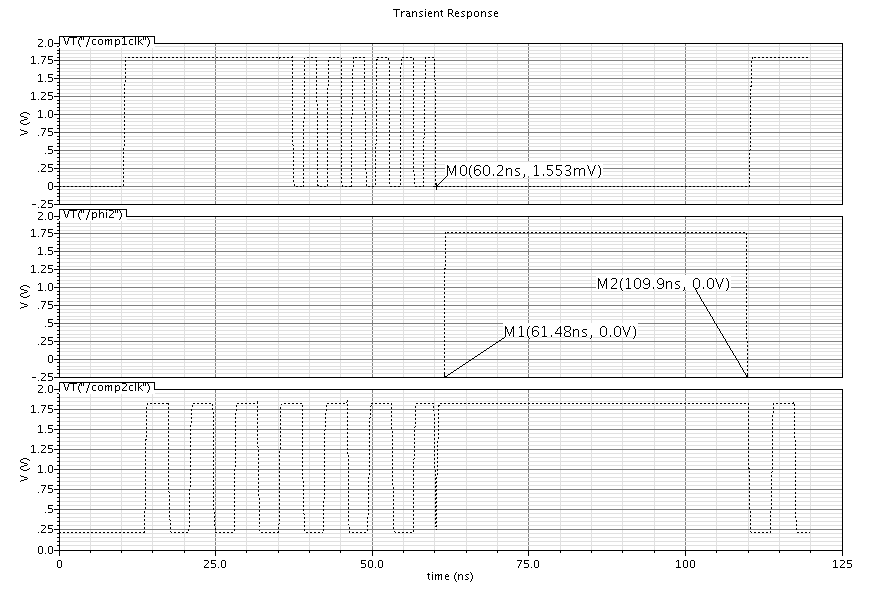
\includegraphics[width=\textwidth]{clockfixes}
\caption{Clocking Modifications Made for Ideal Component Parameter Design}
\label{fig:fixedclocks}
\end{figure}

Once these bugs were fixed, the transient DFT simulation was run on the design. Figure \ref{fig:idealparamsingledft} shows the final DFT output from this iteration of the design. With an SQDR of \SI{74}{\decibel}, this iteration of the design could be considered complete.
\begin{figure}[htbp]
\centering
\includegraphics[width=\textwidth]{ideal_single_two_stage_douttotal_fft}
\caption{Final DFT Output of Single-Ended Model With Ideal OTA Parameters} 
\label{fig:idealparamsingledft}
\end{figure}
\subsection{Simulation with Calculated OTA Model Parameters}
Once the ideal SQDR was achieved with ideal OTA model parameters, the calculated model parameters were used and simulations were run again. In this case, the transient settling simulation and transient DFT simulations were run first. After these simulations, the noise simulations were run to verify the noise behavior of the circuit.

The first verification step was running transient simulations. Figure \ref{fig:singleendedtran} shows the output voltage of the MDAC during the amplification stage with full-scale voltage input. At the end of the amplification phase, the MDAC output voltage is \SI{848.5}{\milli\volt}
\begin{figure}[htbp]
\centering
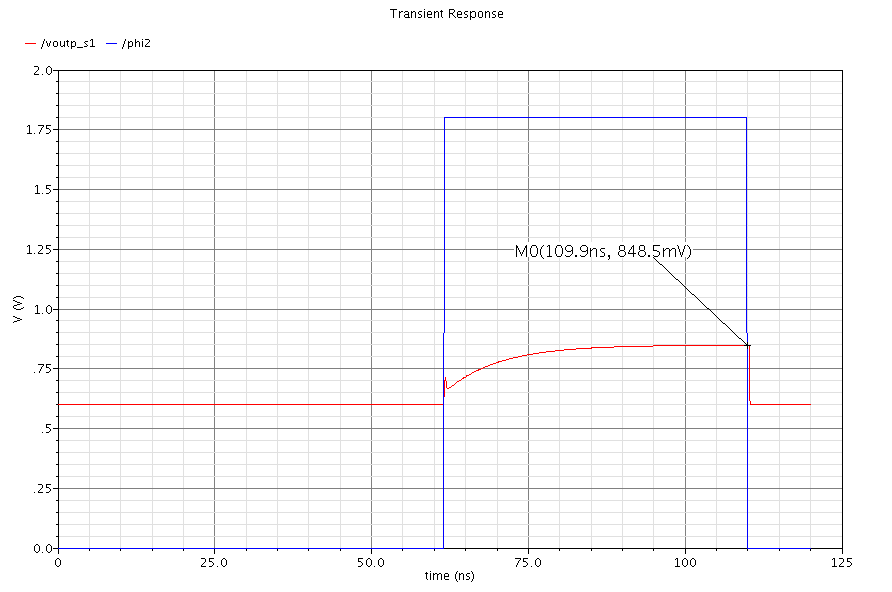
\includegraphics[width=\textwidth]{transingle}
\caption{Transient Settling of Single-Ended ADC With Ideal Components} 
\label{fig:singleendedtran}
\end{figure}
 With a full-scale input, the expected MDAC output is:
\begin{equation}
\label{eq:fullscalemdacoutput}
V_{MDAC} = \dfrac{V_{ref}}{4} + V_{cm}
\end{equation}
where $V_{cm}$ is the common-mode voltage. In this case, the common-mode voltage is set to \SI{600}{\milli\volt}, the expected output voltage is \SI{850}{\milli\volt}. From Figure \ref{fig:singleendedtran}, the settling error is \SI{-1.5}{\milli\volt}. The maximum error is the sum of the static and dynamic error specifications, or \SI{2.4}{\milli\volt}. The full-scale input error was within this error envelope, so the testing moved on to transient DFT.

The initial transient DFT simulation yielded an SQDR of 74 dB, which met the required specification. After achieving this metric, the switch resistances were increased in order to reduce the size and power consumption of the switches when implemented as transistors. After running a number of times, a sampling switch resistance of \SI{400}{\ohm} was found to still produce SQDR. All other switch resistances were set to \SI{500}{\ohm}. Figure \ref{fig:idealsingletwostagecalcparams} shows the final DFT from these simulation runs.
\begin{figure}[htbp]
\centering
\includegraphics[width=\textwidth]{idealsinglecalparamsdft}
\caption{DFT of Single-Ended ADC With Calculated Parameters} 
\label{fig:idealsingletwostagecalcparams}
\end{figure}

After obtaining an SQDR of 74 dB from the transient DFT simulation, noise simulations could be run. First the AC sampling and amplification phase noise simulations were run. Figures \ref{fig:acsamplenoisesingle} and \ref{fig:acholdnoisesingle} are graphs of the integrated output noise obtained from these simulations.
\begin{figure}[htbp]
\centering
\includegraphics[width=\textwidth]{acsamplenoisesingle}
\caption{AC Noise During Sampling Phase of Single-Ended ADC} 
\label{fig:acsamplenoisesingle}
\end{figure}
\begin{figure}[htbp]
\centering
\includegraphics[width=\textwidth]{acholdnoisesingle}
\caption{AC Noise During Amplification Phase of Single-Ended ADC} 
\label{fig:acholdnoisesingle}
\end{figure}
Additionally, an AC noise simulation was run with the OTA noise generator turned off, in order to compare the calculated OTA noise power to that of the simulation. These results are summarized in Table \ref{tab:acnoisesummarysingle}.
\begin{table}[htbp]
\renewcommand*\arraystretch{1.3}
\begin{center}
\begin{tabularx}{\linewidth}{|l|X|X|X|X|}
\hline
Setup & AC Sampling Noise (\si{\milli\volt_{rms}}) & Total AC Hold Noise  (\si{\milli\volt_{rms}}) & AC Hold OTA Noise  (\si{\milli\volt_{rms}}) & AC Total Noise  (\si{\milli\volt_{rms}}) \\ \hline
Simulation & 1.07 & 0.44 & 0.32 & 1.16 \\ \hline
Calculation & 1.07 & 0.41 & 0.33 & 1.10 \\ \hline
Design Target & 1.07 & 1.56 & 1.51 & 1.89 \\ \hline
Error (\%) & 0.31 & 7.10 & -1.69 & 5.63 \\ \hline
Headroom (\%) & -0.48 & 72.20 & 78.66 & 38.89 \\ \hline
\end{tabularx}
\end{center}
\caption{Single-Ended AC Output Noise Power Summary}
\label{tab:acnoisesummarysingle}
\end{table}
The only noise value that significantly diverges from its calculated value is that of the AC hold phase noise, despite the OTA noise being very close to its calculated value. It was first thought that the $C_{s2}$ noise contribution may not have been calculated correctly. To test this, all noise sources were turned off except for the switch at the output of the stage two capacitive array. The output noise in this case matched the calculated kT/C noise, so this was determined to not be the cause of error. Further simulations revealed that the switch resistances at the input of the MDAC were contributing significant noise, which was not accounted for in the noise calculations. Since both the hold noise power and the total noise power were well within their budgets, the switch resistance was not changed as a result of this finding. While no changes were made, the switch resistance was kept as a knob to tune the total output noise power if, after implementing the transistor level design, total output noise became an issue. Next, a PSS/PNOISE simulation was run to verify the AC noise simulations. Figure \ref{fig:pnoisesingle} shows the integrated root-mean-square (RMS) output noise voltage from this simulation. 
\begin{figure}[htbp]
\centering
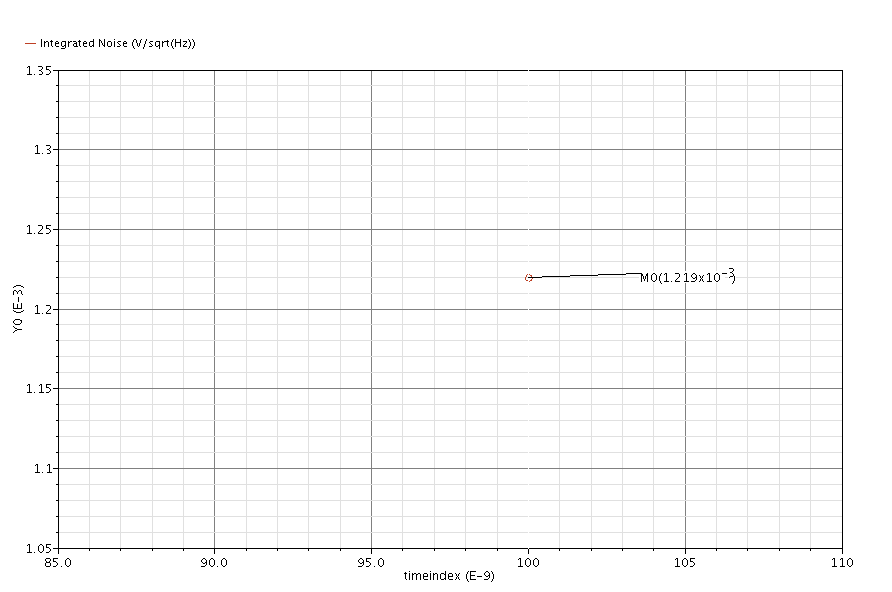
\includegraphics[width=\textwidth]{pnoisesingle}
\caption{Single-Ended PNOISE Simulation Result} 
\label{fig:pnoisesingle}
\end{figure}
Table \ref{tab:pnoisesummarysingle} translates this result into an output noise power and compares it to that from the AC simulations.
\begin{table}[htbp]
\begin{center}
\begin{tabularx}{\linewidth}{|l|X|X|X|}
\hline
Setup & Total Noise Power (\si{\milli\volt_{rms}}) & Error vs Calculation (\%) & Error vs AC Simulation (\%) \\ \hline
PNOISE Simulations & 1.22 & 6.69 & 5.44 \\ \hline
\end{tabularx}
\end{center}
\caption{Single-Ended PNOISE Output Noise Summary}
\label{tab:pnoisesummarysingle}
\end{table}
The PNOISE simulations show good agreement with both the AC Simulations and the calculations. With good agreement between both simulations and the calculations, as well as a total output noise power that was well within budget, the noise simulations were considered a success.

With both noise simulations and transient performance simulations complete, a full SNDR of the single-ended system could be calculated. Solving for the distortion and quantization noise power in Equation \ref{eq:sqdr} yields: 
\begin{align}
\label{eq:pqplusdissingle}
P_{qnoise}+P_{distortion} &= \dfrac{\dfrac{1}{2}\left(\dfrac{V_{FS}}{2}\right)^{2}}{SQDR} \\
\nonu &= \SI{4.94}{\square\nano\volt}
\end{align}
Since the PNOISE result gave the highest output noise, that was the value used for the SNDR calculation. Referring the noise power to the input produced a noise power of \SI{5.82}{\square\nano\volt}. Using Equation \ref{eq:sndr}, the calculated SNDR was:
\begin{equation}
\label{eq:sndrsingle}
SNDR_{SE} = \SI{70.7}{\decibel}
\end{equation}
From Equation \ref{eq:enob}, this translates to an ENOB of 11.4 bits. 
\section{Design of Fully Differential ADC With Ideal Components}
Once the single-ended design was complete, it needed to be expanded to a differential design. Expanding to a differential design involved mirroring the sub-ADC capacitor arrays to enable a positive and negative input, as well as using the differential OTA model for the MDAC. In addition, to accommodate the differential design, the SAR control logic had to be slightly redesigned. The parameters for all of the design blocks and all of the capacitor sizes were able to remain the same, however. The differential design followed a similar design cycle as that of the single-ended design. 
\subsection{Expanding the SAR ADCs to Accept Differential Inputs}
In order for the SAR ADC to accept a differential signal, the voltage reference had to be split into a positive reference voltage and a negative reference voltage. The relationship between these voltages is:
\begin{equation}
\label{eq:vrefp}
V_{refp} = V_{cm}+\dfrac{V_{ref}}{2}
\end{equation}
\begin{equation}
\label{eq:vrefn}
V_{refn} = V_{cm}-\dfrac{V_{ref}}{2}
\end{equation}
Figure \ref{fig:diffsaradc} is an expansion of \ref{fig:saradcdummylsb} to include differential inputs. While Figure \ref{fig:diffsaradc} still uses the dummy LSB capacitor to achieve an extra bit of resolution, the resolution of the ADC has been lowered to two bits. 
\begin{figure}[htbp]
\centering
\newcommand{\colspacing}{4.5}
\newcommand{\colfourspacing}{2}
\newcommand{\rowspacing}{-1}
\newcommand{\negrowspacing}{1}
\newcommand{\digitalrel}{-0.5}
\newcommand{\switchrelctl}{-0.1}
\newcommand{\switchrelspace}{-1}
\newcommand{\labelrelspace}{-1}
\newcommand{\rowone}{0}
\newcommand{\rowtwo}{\rowone+\rowspacing}
\newcommand{\rowthree}{\rowtwo+\rowspacing}
\newcommand{\rowthreehalf}{\rowthree+\rowspacing}
\newcommand{\rowfour}{\rowthreehalf+\rowspacing}
\newcommand{\rowfive}{\rowfour+\rowspacing}
\newcommand{\rowsix}{\rowfive+\rowspacing}
\newcommand{\rowseven}{\rowsix+\rowspacing}
\newcommand{\roweight}{\rowseven+\rowspacing}
\newcommand{\rownine}{\roweight+\rowspacing}
\newcommand{\rowten}{\rownine+\rowspacing}
\newcommand{\roweleven}{\rowten+\rowspacing}
\newcommand{\rowtwelve}{\roweleven+\rowspacing}
\newcommand{\colone}{-2}
\newcommand{\coltwo}{\colone+\colspacing}
\newcommand{\colthree}{\coltwo+\colspacing}
\newcommand{\colfour}{\colthree+\colfourspacing}
\newcommand{\colfive}{\colfour+\colfourspacing}
\newcommand{\colsix}{\colfive+\colfourspacing}
\begin{circuitikz} 
\draw
%in connection
	(\colone, \rowone) node[anchor=south] {$V_{inp}$} -- (\colthree, \rowone)
%vcm connection
	(\colone, \rowtwo) node[anchor=south]  {$V_{cm}$} -- (\colfour+\switchrelspace, \rowtwo)
%vrefp connection
	(\colone, \rowthree) node[anchor=south]  {$V_{refp}$} -- (\coltwo+2*\switchrelspace, \rowthree)
%vrefn connection
	(\colone, \rowthreehalf) node[anchor=south] {$V_{refn}$} -- (\coltwo+3*\switchrelspace, \rowthreehalf)
%bit1 switch connections
	%sample switch
	(\coltwo, \rowfour)  to[cspst, l=$S$] (\coltwo, \rowfive)
	(\coltwo, \rowfour) to [short, -*] (\coltwo, \rowone)
	%vcm switch
	(\coltwo, \rowfour) ++(\switchrelspace, 0) to [cspst, l=$G$]  ++(0, \rowspacing) to [short, -*] ++(0,0)
	(\coltwo, \rowfour) ++(\switchrelspace, 0) to [short, -*] ++(0, -3*\rowspacing)
	%vrefp switch
	(\coltwo, \rowfour) ++(2*\switchrelspace, 0) to [cspst, l=$d_{1}$]  ++(0, \rowspacing) to [short, *-] ++(0, 0) 
	(\coltwo, \rowfour) ++(2*\switchrelspace, 0) to [short] ++(0, -2*\rowspacing)
	(\coltwo, \rowfive) -- ++(2*\switchrelspace, 0)
	%vrefn switch
	(\coltwo, \rowfour) ++(3*\switchrelspace, 0) to [cspst, l=$\overline{d_{1}}$]  ++(0, \rowspacing)
	(\coltwo, \rowfour) ++(3*\switchrelspace, 0) to [short] ++(0, -1*\rowspacing)
	(\coltwo, \rowfive) -- ++(3*\switchrelspace, 0)
%bit1 cap
	(\coltwo, \rowfive) ++(\switchrelspace, 0) to [C, l=C] ++(0, \rowspacing)
%dummy LSB switch connections
	%sample switch
	(\colthree, \rowfour)  to[cspst, l=$S$] (\colthree, \rowfive)
	(\colthree, \rowfour) to [short] (\colthree, \rowone)
	%vcm switch
	(\colthree, \rowfour) ++(\switchrelspace, 0) to [cspst, l=$G$]  ++(0, \rowspacing) to [short, -*] ++(0,0) 
	(\colthree, \rowfour) ++(\switchrelspace, 0) to [short, -*] ++(0, -3*\rowspacing)
	%vrefp switch
	(\colthree, \rowfour) ++(2*\switchrelspace, 0) to [cspst, l=$d_{0}$]  ++(0, \rowspacing) to [short, *-] ++(0, 0) 
	(\colthree, \rowfour) ++(2*\switchrelspace, 0) to [short] ++(0, -2*\rowspacing)
	node[anchor=south] {$V_{refp}/2$}
	(\colthree, \rowfive) -- ++(2*\switchrelspace, 0)
	%vrefn switch
	(\colthree, \rowfour) ++(3*\switchrelspace, 0) to [cspst, l=$\overline{d_{0}}$]  ++(0, \rowspacing)
	(\colthree, \rowfour) ++(3*\switchrelspace, 0) to [short] ++(0, -1*\rowspacing)
	node[anchor=south] {$V_{refn}/2$}
	(\colthree, \rowfive) -- ++(3*\switchrelspace, 0)
%dummy lsb cap
	(\colthree, \rowfive) ++(\switchrelspace, 0) to [C, l=C] ++(0, \rowspacing)  to [short, *-] ++(0, 0)
	(\colthree, \rowfive) -- ++(\switchrelspace, 0)
%comp input vcm switch
	(\colfour, \rowfour) ++(\switchrelspace, 0) to [cspst, l=$S$]  ++(0, \rowspacing)
	(\colfour, \rowfour) ++(\switchrelspace, 0) to [short] ++(0, -3*\rowspacing)
	(\colfour, \rowfive) ++(\switchrelspace, 0) -- ++(0, \rowspacing)  to [short, -*] ++(0,0)
	(\coltwo+\switchrelspace, \rowsix) -- (\colfour, \rowsix)
	node[plain amp, anchor=-] (comp) {}
	(comp.-) ++(-0.5, 0) node[anchor=south west] {X}
	(comp.center) ++(-0.1,0) node[anchor=center] {Comp}
	(comp.out) node[anchor=south] {$d_{n}$}
%neg comp input vcm switch
	(comp.+) ++(-0.5, 0) node[anchor=south west] {Y} -- (\colfour, \rowseven) --
	++(\switchrelspace, 0) to [short, *-] ++(0,-1*\negrowspacing) to [cspst, l=$S$] ++(0, -1*\negrowspacing)
	(\colfour, \roweight) ++(\switchrelspace, 0) to [short] ++(0, -3*\negrowspacing)
	(\colfour, \rowfive) ++(\switchrelspace, 0) -- ++(0, \negrowspacing)
	(\coltwo+\switchrelspace, \rowseven) -- (\colfour, \rowseven)
%in connection
	(\colone, \rowtwelve) node[anchor=south] {$V_{inn}$} -- (\colthree, \rowtwelve)
%vcm connection
	(\colone, \roweleven) node[anchor=south]  {$V_{cm}$} -- (\colfour+\switchrelspace, \roweleven)
%vrefn connection
	(\colone, \rowten) node[anchor=south]  {$V_{refn}$} -- (\coltwo+2*\switchrelspace, \rowten)
%vrefp connection
	(\colone, \rownine) node[anchor=south] {$V_{refp}$} -- (\coltwo+3*\switchrelspace, \rownine)
%dummy LSB switch connections
	%sample switch
	(\colthree, \roweight)  to[cspst, l=$S$] (\colthree, \rownine)
	(\colthree, \roweight) to [short] (\colthree, \rowtwelve)
	%vcm switch
	(\colthree, \roweight) ++(\switchrelspace, 0) to [short, -*] ++(0,0) to [cspst, l=$G_{1}$]  ++(0, -\negrowspacing)
	(\colthree, \roweight) ++(\switchrelspace, 0) to [short, -*] ++(0, -3*\negrowspacing)
	%vrefn switch
	(\colthree, \roweight) ++(2*\switchrelspace, 0) to [short, *-] ++(0, 0) to [cspst, l=$d_{0}$]  ++(0, -1*\negrowspacing)
	(\colthree, \roweight) ++(2*\switchrelspace, 0) to [short] ++(0, -2*\negrowspacing)
	node[anchor=north] {$V_{refn}/2$}
	(\colthree, \roweight) -- ++(2*\switchrelspace, 0)
	%vrefp switch
	(\colthree, \roweight) ++(3*\switchrelspace, 0) to [cspst, l=$\overline{d_{0}}$]  ++(0, -1*\negrowspacing)
	(\colthree, \roweight) ++(3*\switchrelspace, 0) to [short] ++(0, -1*\negrowspacing)
	node[anchor=north] {$V_{refp}/2$}
	(\colthree, \roweight) -- ++(3*\switchrelspace, 0)
%dummy lsb cap
	(\colthree, \rowseven) ++(\switchrelspace, 0) to [C, l=C] ++(0, -\negrowspacing)
	(\colthree, \rowseven) -- ++(\switchrelspace, 0)
%bit1 switch connections
	%sample switch
	(\coltwo, \roweight)  to[cspst, l=$S$] (\coltwo, \rownine)
	(\coltwo, \roweight) to [short, -*] (\coltwo, \rowtwelve)
	%vcm switch
	(\coltwo, \roweight) ++(\switchrelspace, 0) to [short, -*] ++(0,0) to [cspst, l=$G_{0}$]  ++(0, -\negrowspacing)
	(\coltwo, \roweight) ++(\switchrelspace, 0) to [short, -*] ++(0, -3*\negrowspacing)
	%vrefn switch
	(\coltwo, \roweight) ++(2*\switchrelspace, 0) to [short, *-] ++(0, 0) to [cspst, l=$d_{1}$]  ++(0, -\negrowspacing)
	(\coltwo, \roweight) ++(2*\switchrelspace, 0) to [short] ++(0, -2*\negrowspacing)
	(\coltwo, \roweight) -- ++(2*\switchrelspace, 0)
	%vrefp switch
	(\coltwo, \roweight) ++(3*\switchrelspace, 0) to [cspst, l=$\overline{d_{1}}$]  ++(0, -\negrowspacing)
	(\coltwo, \roweight) ++(3*\switchrelspace, 0) to [short] ++(0, -1*\negrowspacing)
	(\coltwo, \roweight) -- ++(3*\switchrelspace, 0)
%bit1 cap
	(\coltwo, \roweight) ++(\switchrelspace, 0) to [C, l=C] ++(0, \negrowspacing)
;
\end{circuitikz}
\caption{Example Two Bit Differential SAR ADC}
\label{fig:diffsaradc}
\end{figure}
The switches connecting the bottom plate of the sampling capacitors is now controlled by a new signal, $G$. At the end of the sampling phase, the $G$ signal is asserted for all bits, and all other switches are open. Using an analysis similar to the analysis from Section \ref{sec:saroperation}, the expression for the comparator output at the end of the first conversion step is:
\begin{equation}
\label{sard1diff}
d_{n} =	\begin{cases}
				0 & \mbox{if } V_{inp} > V_{inn} \\[0.5em]
				1 & \mbox{if } V_{inp} < V_{inn}
			\end{cases}
\end{equation}
Once again, the digital output of the ADC is the logical not of the comparator output. After the first conversion step, $G_{1}$ is deasserted, and the expression for the differential voltage at the comparator inputs is:
\begin{equation}
\label{eq:vdiffsarout}
V_{diff,cin} = \begin{cases}
				(V_{inp}-V_{inn}) - \dfrac{V_{ref}}{2} & \mbox{if } d_{1} = 1 \\[0.5em]
				(V_{inp}-V_{inn}) + \dfrac{V_{ref}}{2} & \mbox{if } d_{1} = 0
			\end{cases}
\end{equation}
The expression for the $d_{0}$ at the end of the second conversion stage is:
\begin{equation}
d_{0} =	\begin{cases}
				1 & \mbox{if } V_{inp}-V_{inn} > \dfrac{\pm V_{ref}}{2} \\[0.5em]
				0 & \mbox{if } V_{inp}-V_{inn} < \dfrac{\pm V_{ref}}{2}
			\end{cases}
\end{equation}
where $V_{ref}$ is positive if $d_{1}$ is 1 and negative if $d_{1}$ is 0. Conversion could continue in this manner for an arbitrary number of stages. 
\subsection{Design of Differential Control Logic}
The expansion to differential outputs necessitated two major changes in the SAR control logic. First, a new control signal has been added to control the switches connected to the common-mode input. These switches must stay asserted until after the corresponding bit decision stage. Additionally, the first decision stage of the differential ADC requires that only $G_{i}$ signals be asserted, which is different than that of the single-ended stage.  In addition to these required changes, some design issues that were encountered during the single-ended design phase needed to be addressed. The reason the additional clock cycle needed to be added to the second-stage ADC is that the state machine was being asynchronously reset by the rising edge of the sampling clock signal. This asynchronous behavior was removed during the design of the differential control logic. The state machine would now reset itself synchronously, so issues between the clock domains were removed and the second stage sampling clock frequency could be restored to \SI{140}{\mega\hertz}. Also, flip-flops separate from the normal control logic were used to store the digital output codes, allowing for easier sampling of the digital data. 

Table \ref{tab:statemachinedoutdiff} shows the digital outputs, $d_{i}$, in terms of the differential SAR state machine. Table \ref{tab:statemachinegdiff} shows the common-mode switch control output, $G$, in terms of the differential SAR state machine. The $G_{i}$, $d_{i}$, and $\overline{d_{i}}$, control signals must all be gated by the sampling clock of the sub-ADC, so that only the input sampling switch is closed during the sampling phase. The first and second stage control logic had only two differences. First the the second stage has an extra state to account for the extra conversion step required. Second, the sampling clock and the SAR conversion clocks for the two stages are different, although the internal behavior in response to these clocks is exactly the same. At the first falling edge of the SAR conversion clock, the state machine moves from state 6, or 7, to state 0 and conversion begins. Conversion ends when the state machine reaches state 6, or 7.
\begin{table}[htbp]
\renewcommand*\arraystretch{1.3}
\begin{center}
\begin{tabular}{|r|r|r|r|l|r|r|r|}
\hline
\multicolumn{1}{|l|}{Current State} & \multicolumn{1}{l|}{Next State} & \multicolumn{1}{l|}{$d_{5}$} & \multicolumn{1}{l|}{$d_{4}$} & $d_{3}$ & \multicolumn{1}{l|}{$d_{2}$} & \multicolumn{1}{l|}{$d_{1}$} & \multicolumn{1}{l|}{$d_{0}$} \\ \hline
0 & 1 & 0 & 0 & \multicolumn{1}{r|}{0} & 0 & 0 & 0 \\ \hline
1 & 2 & $\overline{C}$ & 0 & \multicolumn{1}{r|}{0} & 0 & 0 & 0 \\ \hline
2 & 3 & $d_{5p}$ & $\overline{C}$ & \multicolumn{1}{r|}{0} & 0 & 0 & 0 \\ \hline
3 & 4 & $d_{5p}$ & $d_{4p}$ & \multicolumn{1}{r|}{$\overline{C}$} & 0 & 0 & 0 \\ \hline
4 & 5 & $d_{5p}$ & $d_{4p}$ & $d_{3p}$ & $\overline{C}$ & 0 & 0 \\ \hline
5 & 6 & $d_{5p}$ & $d_{4p}$ & $d_{3p}$ & \multicolumn{1}{l|}{$d_{2p}$} & $\overline{C}$ & 0 \\ \hline
6 & 7 & $d_{5p}$ & $d_{4p}$ & $d_{3p}$ & \multicolumn{1}{l|}{$d_{2p}$} & \multicolumn{1}{l|}{$d_{1p}$} & $\overline{C}$ \\ \hline
\end{tabular}
\end{center}
\caption{Differential ADC Digital Output State Machine}
\label{tab:statemachinedoutdiff}
\end{table}

\begin{table}[htbp]
\begin{center}
\begin{tabular}{|r|r|r|r|r|r|r|r|}
\hline
\multicolumn{1}{|l|}{Current State} & \multicolumn{1}{l|}{Next State} & \multicolumn{1}{l|}{$G_{5}$} & \multicolumn{1}{l|}{$G_{4}$} & \multicolumn{1}{l|}{$G_{3}$} & \multicolumn{1}{l|}{$G_{2}$} & \multicolumn{1}{l|}{$G_{1}$} & \multicolumn{1}{l|}{$G_{0}$} \\ \hline
0 & 1 & 1 & 1 & 1 & 1 & 1 & 1 \\ \hline
1 & 2 & 0 & 1 & 1 & 1 & 1 & 1 \\ \hline
2 & 3 & 0 & 0 & 1 & 1 & 1 & 1 \\ \hline
3 & 4 & 0 & 0 & 0 & 1 & 1 & 1 \\ \hline
4 & 5 & 0 & 0 & 0 & 0 & 1 & 1 \\ \hline
5 & 6 & 0 & 0 & 0 & 0 & 0 & 1 \\ \hline
6 & 7 & 0 & 0 & 0 & 0 & 0 & 0 \\ \hline
\end{tabular}
\end{center}
\caption{Common-Mode Switch Control Output State Machine}
\label{tab:statemachinegdiff}
\end{table}
\subsection{Simulation Using Ideal OTA Model Parameters}
Similar to the design of the single-ended ADC, ideal OTA model parameters were used in order to verify the SAR operation. This phase was much shorter than in the single-ended case, as almost all of the bugs that were found were in the control logic and fixing them was straightforward. The amplification phase had to be shortened by another \SI{100}{\pico\second} in order for the last bit decision to fully settle. This slight decrease in the amplification phase did not necessitate any change in the OTA transconductance. By the end of this phase, the SQDR was once again 74 dB.
\subsection{Simulation with Calculated OTA Model Parameters}
After obtaining an ideal SQDR with the ideal OTA model parameters, the design was put through the same battery of tests that the single-ended design was put through. Transient simulations ensured that distortion power did not negatively effect the ADC performance, and then noise simulations were performed to ensure that the output noise was within its budget.

The transient settling simulation was the same as in the single-ended case, except that an input with the maximum negative magnitude and the maximum positive magnitude was used to ensure that the settling was not affected by signal polarity. Figures \ref{fig:tranposdiff} and \ref{fig:trannegdiff} are the graphs of the transient settling with a full-scale positive input and full-scale negative input, respectively.
\begin{figure}[htbp]
\centering
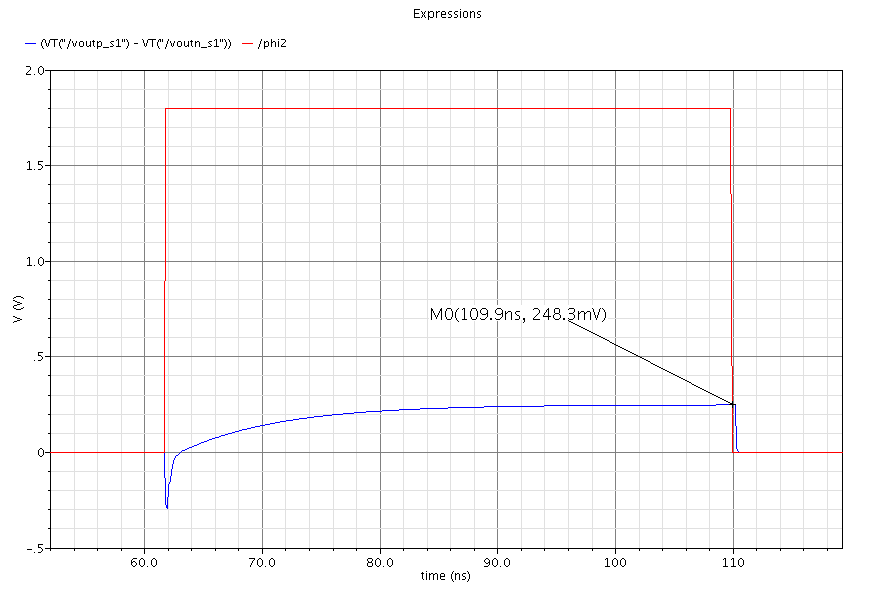
\includegraphics[width=\textwidth]{tranposdiff}
\caption{Transient Settling of Differential ADC With Ideal Components With Full-Scale Positive Input Voltage} 
\label{fig:tranposdiff}
\end{figure}
\begin{figure}[htbp]
\centering
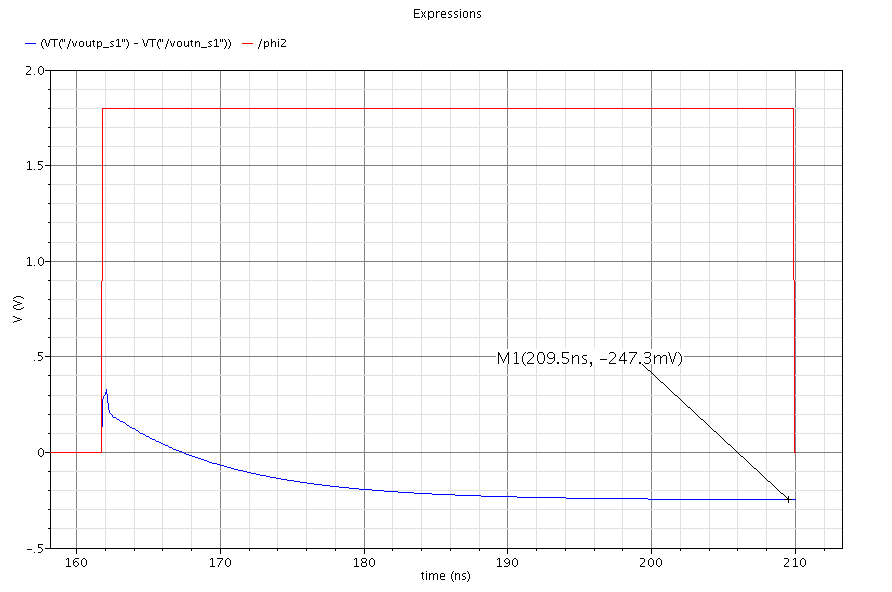
\includegraphics[width=\textwidth]{trannegdiff}
\caption{Transient Settling of Differential ADC With Ideal Components With Full-Scale Negative Input Voltage} 
\label{fig:trannegdiff}
\end{figure}
In the case of the positive input, the settling error is \SI{-1.7}{\milli\volt}. In the case of the negative input, the transient settling error is \SI{2.7}{\milli\volt}. In both of these cases, the settling error is within the maximum settling error envelope.

After verifying that the MDAC was settling properly, the DFT simulations were run. These simulations yielded an SQDR of 74 dB on the first run. Some additional runs were performed, however, to try to adjust the size of the sampling switches. In the case of the differential design, all switches were able to be sized with an on resistance of \SI{500}{\ohm}. Figure \ref{fig:fftfinaldiff} shows the DFT results from the final run of the differential simulation.
\begin{figure}[htbp]
\centering
\includegraphics[width=\textwidth]{ideal_diff_two_stage_douttotal_fft}
\caption{DFT of Differential ADC With Calculated Model Parameters} 
\label{fig:fftfinaldiff}
\end{figure}

With the transient performance meeting specification, the final step in the verification of the differential design was the noise simulations. Graphs of the simulation results from the AC noise simulations are given in Figures \ref{fig:acsamplenoisediff} and \ref{fig:acholdnoisediff}. 
\begin{figure}[htbp]
\centering
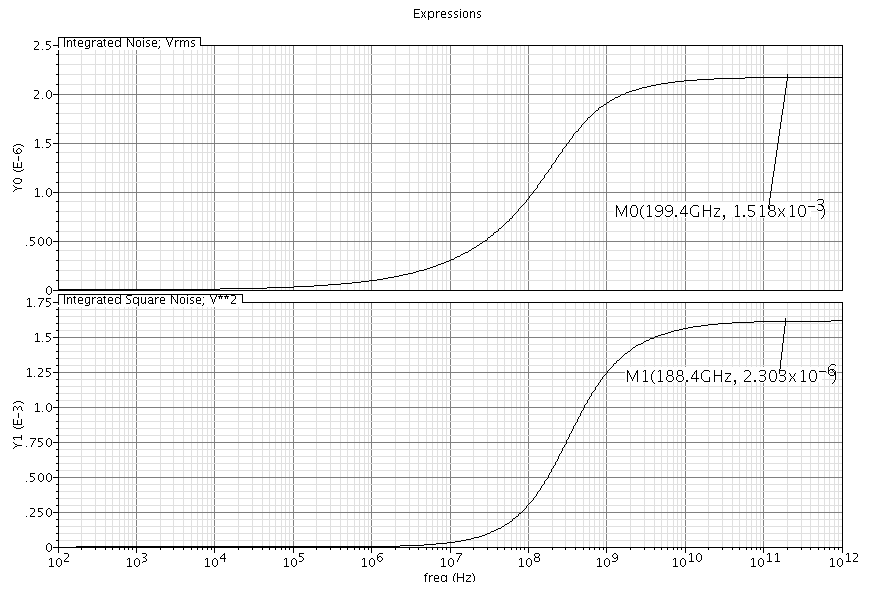
\includegraphics[width=\textwidth]{acsamplenoisediff}
\caption{AC Noise During Sampling Phase of Differential ADC} 
\label{fig:acsamplenoisediff}
\end{figure}
\begin{figure}[htbp]
\centering
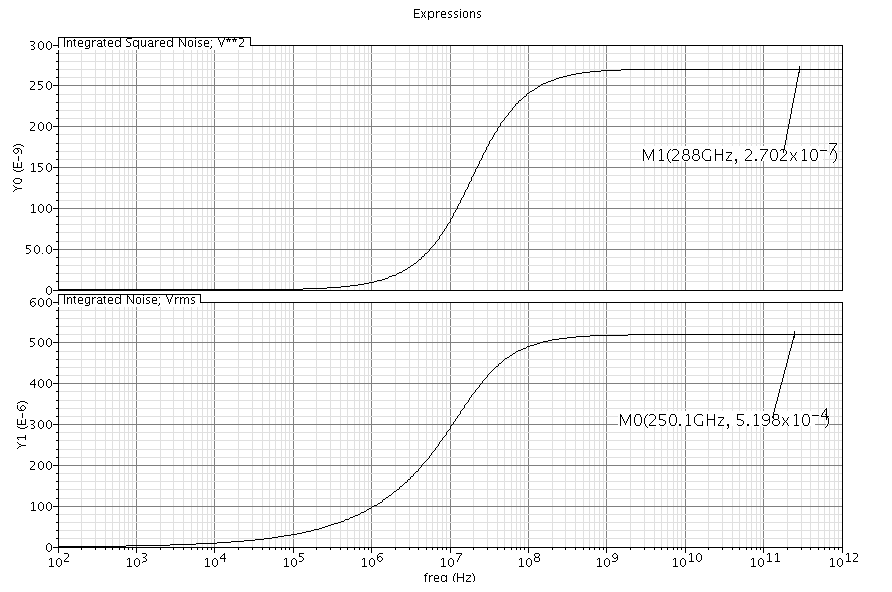
\includegraphics[width=\textwidth]{acholdnoisediff}
\caption{AC Noise During Amplification Phase of Differential ADC} 
\label{fig:acholdnoisediff}
\end{figure}
Not surprisingly, the noise contribution from the sampling phase has roughly doubled. This is due to the doubling of the capacitance from the differential design. The noise in the amplification phase does not exactly double because the OTA noise power is independent of the differential or single-ended implementation. The contribution to amplification phase noise power from the input switches and from the second stage capacitive array does double, however. Table \ref{tab:acnoisesummarydiff} summarizes the results from the AC noise simulation.
\begin{table}[htbp]
\begin{center}
\begin{tabularx}{\linewidth}{|l|X|X|X|X|}
\hline
Setup & AC Sampling Noise (\si{\milli\volt_{rms}}) & Total AC Hold Noise  (\si{\milli\volt_{rms}}) & AC Hold OTA Noise  (\si{\milli\volt_{rms}}) & AC Total Noise  (\si{\milli\volt_{rms}}) \\ \hline
Simulation & 1.52 & 0.52 & 0.32 & 1.60 \\ \hline
Calculation & 1.51 & 0.34 & 0.33 & 1.55 \\ \hline
Design Target & 1.51 & 1.62 & 1.51 & 2.21 \\ \hline
Error (\%) & 0.31 & 53.79 & -1.69 & 3.48 \\ \hline
Headroom (\%) & -0.26 & 67.82 & 78.66 & 27.55 \\ \hline
\end{tabularx}
\end{center}
\caption{Differential AC Output Noise Summary}
\label{tab:acnoisesummarydiff}
\end{table}
Once again, the hold noise calculations are off due to neglecting the contribution to noise power of the input switches. Despite this limitation, the noise power is still well within the budget. Figure \ref{fig:pnoisediff} is the result of the PSS/PNOISE simulation with the differential ADC.
\begin{figure}[htbp]
\centering
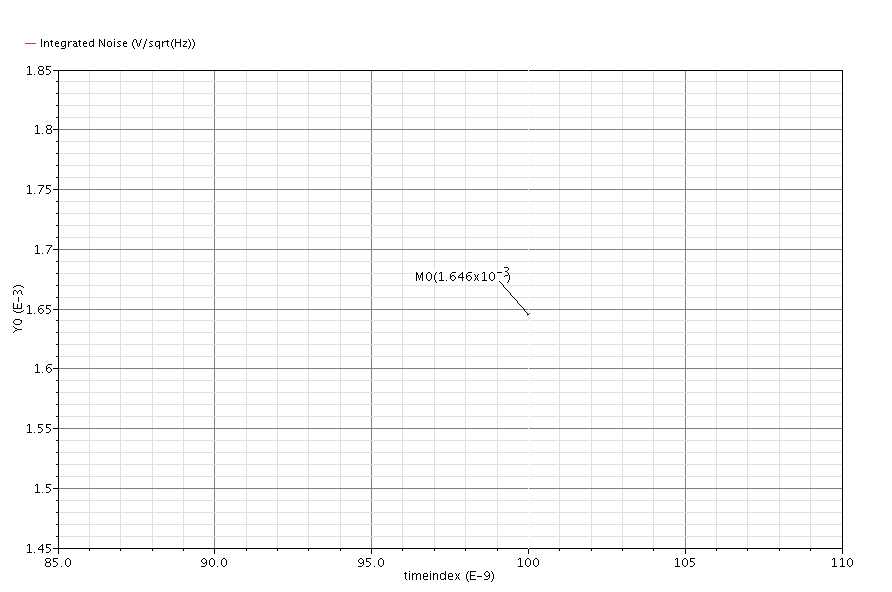
\includegraphics[width=\textwidth]{pnoisediff}
\caption{Differential PNOISE Simulation Result} 
\label{fig:pnoisediff}
\end{figure}
The results from this simulation are compared with the noise calculations and the results from the AC noise simulation in Table \ref{tab:pnoisesummarydiff}. 
\begin{table}[htbp]
\begin{center}
\begin{tabularx}{\linewidth}{|l|X|X|X|}
\hline
Setup & Total Noise Power (\si{\milli\volt_{rms}}) & Error vs Calculation (\%) & Error vs AC Simulation (\%) \\ \hline
PNOISE Simulations & \multicolumn{1}{r|}{1.65} & \multicolumn{1}{r|}{6.21} & \multicolumn{1}{r|}{2.64} \\
\hline
\end{tabularx}
\end{center}
\caption{Differential PNOISE Output Noise Summary}
\label{tab:pnoisesummarydiff}
\end{table}
The differential PNOISE results agreed closely with the calculated results and the AC noise simulations, so the noise simulations were considered successful.

As in the case of the single-ended design, an equivalent SNDR could now be calculated with the SQDR and noise power. The differential PNOISE noise power was used, as this was the largest simulated noise power. The calculated SNDR for the differential design was:
\begin{equation}
\label{eq:sndridealdiff}
SNDR = \SI{72.6}{\decibel}
\end{equation}
From Equation \ref{eq:sndridealdiff}, the ENOB is calculated to be 11.8 bits, which is better than the result from the single-ended design. With the differential ADC design performance meeting specification, the design could move on to the next phase, implementing transistor-level designs for the OTA.